%	Preamble. Put stuff here to define global settings.
% SJK: Document template originally from Andy Maloney "untitled.tex"
\documentclass{article}

%	Packages used.
\usepackage{amsmath}
\usepackage{fullpage}
\usepackage{graphicx}
\usepackage{caption}
\usepackage{subcaption}
%% see: http://en.wikibooks.org/wiki/LaTeX/Floats,_Figures_and_Captions#Subfloats
%	Define new commands for fun and expediated typing.
\newcommand{\bdm}{\begin{displaymath}}
\newcommand{\edm}{\end{displaymath}}

\begin{document}
	Quick summary of learning K-means clustering (2.2.4.1.1. K-means clustering in sklearn tutorial).

	\begin{itemize}
		\item KMeans doc can be found here http://scikit-learn.org/dev/modules/generated/sklearn.cluster.KMeans.html.
		\item By default it uses the k-means++ algorithm for seeding.  This makes sense to me.  I like this stuff because it reminds me a lot of stuff I was doing in grad school around 2000, and it looks like a lot of this machine learning stuff was still being developed back then (i.e. it's newish)
		\item right now, I can't figure out what .squeeze() method does...oh, now i see it's a numpy array thing to get rid of dimensions of size 1: http://docs.scipy.org/doc/numpy/reference/generated/numpy.squeeze.html
	\end{itemize}

    \begin{figure}
            \centering
            \begin{subfigure}[b]{0.3\textwidth}
                    \centering
                    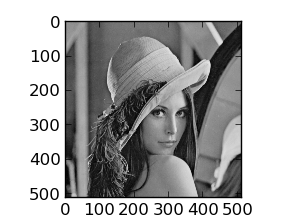
\includegraphics[width=\textwidth]{original.png}
                    \caption{Original image}
                    \label{fig:original3}
            \end{subfigure}%
            ~ %add desired spacing between images, e. g. ~, \quad, \qquad etc.
              %(or a blank line to force the subfigure onto a new line)
            \begin{subfigure}[b]{0.3\textwidth}
                    \centering
                    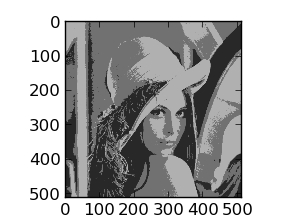
\includegraphics[width=\textwidth]{compressed_3.png}
                    \caption{Binned with kmeans opt.}
                    \label{fig:compressed3}
            \end{subfigure}
            ~ %add desired spacing between images, e. g. ~, \quad, \qquad etc.
              %(or a blank line to force the subfigure onto a new line)
            \begin{subfigure}[b]{0.3\textwidth}
                    \centering
                    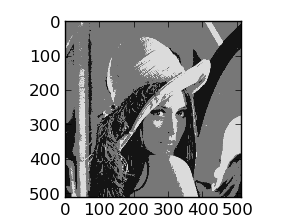
\includegraphics[width=\textwidth]{equal_bins_3.png}
                    \caption{Equally spaced bins}
                    \label{fig:equal_bins3}
            \end{subfigure}
            \caption{colors groups by kmeans, 3 bins}\label{fig:images3}
            
             \begin{subfigure}[b]{0.3\textwidth}
                    \centering
                    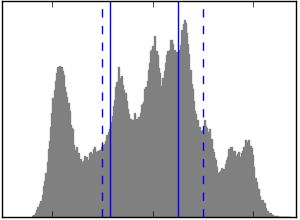
\includegraphics[width=\textwidth]{histogram_3.png}
                    \caption{histogram}
                    \label{fig:histogram3}
            \end{subfigure}
    \end{figure}

    \begin{figure}
            \centering
            \begin{subfigure}[b]{0.3\textwidth}
                    \centering
                    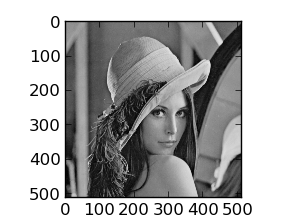
\includegraphics[width=\textwidth]{original.png}
                    \caption{Original image}
                    \label{fig:original5}
            \end{subfigure}%
            ~ %add desired spacing between images, e. g. ~, \quad, \qquad etc.
              %(or a blank line to force the subfigure onto a new line)
            \begin{subfigure}[b]{0.3\textwidth}
                    \centering
                    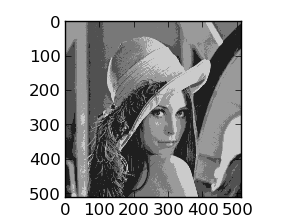
\includegraphics[width=\textwidth]{compressed_5.png}
                    \caption{Binned with kmeans opt.}
                    \label{fig:compressed5}
            \end{subfigure}
            ~ %add desired spacing between images, e. g. ~, \quad, \qquad etc.
              %(or a blank line to force the subfigure onto a new line)
            \begin{subfigure}[b]{0.3\textwidth}
                    \centering
                    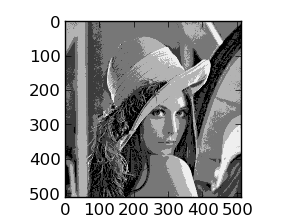
\includegraphics[width=\textwidth]{equal_bins_5.png}
                    \caption{Equally spaced bins}
                    \label{fig:equal_bins5}
            \end{subfigure}
            
            \begin{subfigure}[b]{0.3\textwidth}
                    \centering
                    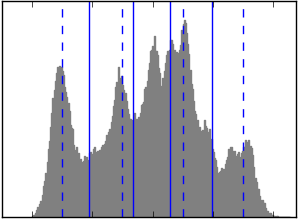
\includegraphics[width=\textwidth]{histogram_5.png}
                    \caption{histogram}
                    \label{fig:histogram5}
            \end{subfigure}
            \caption{colors groups by kmeans, 5 bins}\label{fig:images5}
    \end{figure}
\begin{itemize}

    \item	3 bins: Figure \ref{fig:images3}.
    \item   5 bins: Figure \ref{fig:images5}
	
\end{itemize}

\end{document}
